\documentclass[11pt, a4paper]{article}
\usepackage{graphicx}
\usepackage{amsmath}
\usepackage{listings}

\title{Assignment 3: Fitting Data to Models} % Title
\author{Harshavardhan Mudadala\\
			EE20B084} % Author name
\date{\today} % Date for the report

\begin{document}
\maketitle % Insert the title, author and date

\section*{Q1:Solution}
Get the "fitting.dat" file by running generate$\_$data.py

\section*{Q2:Solution}
Load fitting.dat file using following code
\begin{verbatim}	
import numpy as np

data_table = np.loadtxt('fitting.dat')
t = c_[data_table[:,0]]
N,k = shape(data_table)
print(N,k)
\end{verbatim} 

\section*{Q3:Solution}
The data columns correspond to the function with different amounts of noise added.\\
\begin{equation*}
 f(t) = 1.05J_{2}(t)-0.105t+n(t)
\end{equation*}
\begin{equation*}
 sigma = logspace(-1,-3,9)
\end{equation*}

\section*{Q4:Solution}
Model Function for this data 
\begin{equation*}
 g(t; A, B) = AJ_{2}(t) + Bt
\end{equation*}
\begin{figure}[!tbh]
   	\centering
   	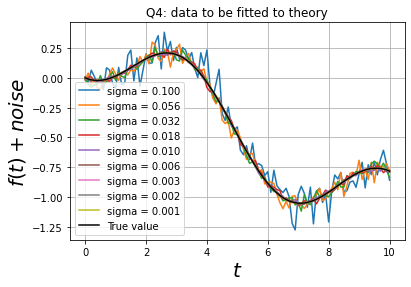
\includegraphics[scale=0.5]{Q4plot.png}  % Mention the image name within the curly braces. Image should be in the same folder as the tex file. 
   	\caption{Data to be fitted to theory}
   \end{figure} 

\section*{Q5:Solution}
A plot of the first column(sigma = 0.1) of data with error bars with every 5th data item to make the plot readable.Use following command to plot error bars.
\begin{equation*}
 errorbar(t[::5],data[::5],stdev,fmt=’ro’)
\end{equation*}
\begin{figure}[!tbh]
   	\centering
   	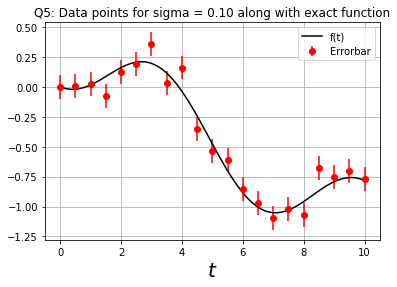
\includegraphics[scale=0.5]{Q5plot.png}  % Mention the image name within the curly braces. Image should be in the same folder as the tex file. 
   	\caption{Data points for sigma = 0.10 along with exact function}
\end{figure} 

\section*{Q6:Solution}
g(t, A, B) = M.p \\
Construct M and inorder confirm two vectors are equal, confirm their elements must be equal

\section*{Q7:Solution}
For A = 0, 0.1, . . . , 2 and B = -0.2, -0.19, . . . , 0, compute "mean squared error" 
\begin{equation}
  \epsilon_{ij} = \frac{1}{101}\sum_{k=0}^{101}(f_k - g(t_k, A_i, B_j))^2)
\end{equation}

\section*{Q8:Solution}
countour plot of $\epsilon_{ij}$ with B on Y-axis and A on X-axis.
\begin{figure}[!tbh]
  \centering
  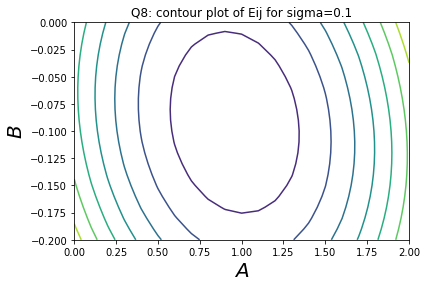
\includegraphics[scale=0.5]{Q8plot.png}  
  \caption{contour plot of $\epsilon_{ij}$ for sigma = 0.1}
\end{figure}

\section*{Q9:Solution}
Use the Python function "lstsq" from "scipy.linalg" to obtain the best estimate of A and B.\\
Use following Code
\begin{verbatim}
Aerr = np.zeros(k)
Berr = np.zeros(k)
from scipy.linalg import lstsq
for i in range(k):
  p,resid,rank,sig=lstsq(M,c_[data_table[:,i+1]])
  Aerr[i] = abs(p[0] - 1.05)
  Berr[i] = abs(p[1] - (-0.105))
\end{verbatim}

\section*{Q10:Solution}
Repeating this with the different columns (i.e., columns 1 and i).
\begin{figure}[!tbh]
  \centering
  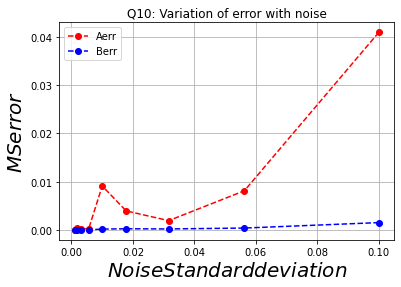
\includegraphics[scale=0.5]{Q10plot.png}  
  \caption{Variation of error with noise}
\end{figure}

\section*{Q11:Solution}
Replotting the above curves using loglog.
\begin{figure}[!tbh]
  \centering
  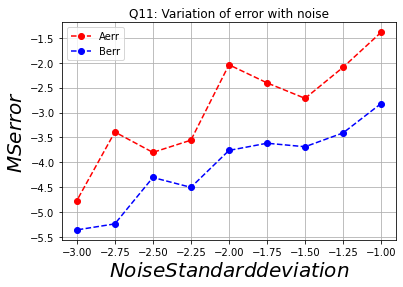
\includegraphics[scale=0.5]{Q11plot.png}  
  \caption{Variation of error with noise using loglog scale}
\end{figure}

From the graph we can see that error is approximately linear with $\sigma$ in the log scale.
\end{document}